\newpage
\section{Alarmliste}
\thispagestyle{fancy}

Alarmhandtering har ikkje blitt implementert i programmet da dette er noko som naturleg ville blitt programmert heilt til slutt,
og tiden strakk ikkje til slik at vi kunne gjennomføre alle krav og måla vi hadde satt oss.
Dette er alarmane som er på anlegget per dags dato

\begin{figure}[htbp]
    \centering
    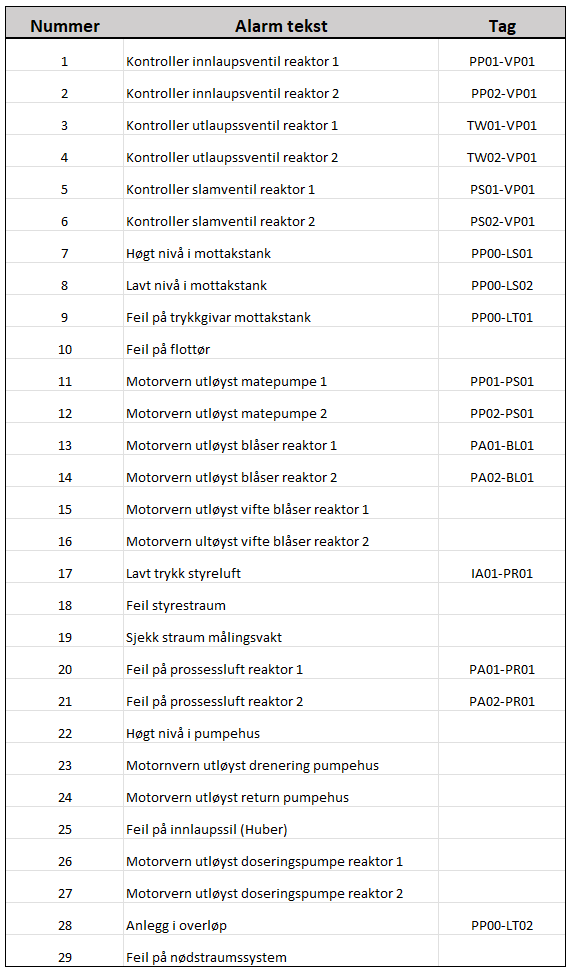
\includegraphics[width=0.6\textwidth]{Bilder/Gammal_Alarmliste.png}
    \caption{Eksisternade alarmliste}\label{fig:reaktorsoner}
\end{figure}

\newpage

IEC blokkene som vi har programmert gir oss også moglegheiten til å implimentere fleire alarmar til anlegget.
Blokkene som vi har programmert har tilgang til desse ekstra feilmeldingane:

\textbf{MA:}
    \begin{itemize}
        \item Feil på blokk
    \end{itemize}
\textbf{MB:}
    \begin{itemize}
        \item Feil på blokk
    \end{itemize}
\textbf{SBE:}
    \begin{itemize}
        \item Ekstern feil
        \item Tap av inngang XE
        \item Tilbakemeldings feil
        \item Safeguarding feil
    \end{itemize}

\textbf{SBV:}
    \begin{itemize}
        \item Ekstern feil
        \item Max opnetid utløpt
        \item Max stengetid utløpt
        \item Både XHG og XGL tilbakemelding høg
        \item Mista tilbakemelding XGH når ventil open
        \item Mista tilbakemelding XGL når ventil stengt
        \item Safeguarding feil
    \end{itemize}

\newpage